% #################################################
% Welcome to the LaTeX template file of Computer-Aided Design and Applications! 
% Please follow the instructions in this document to write and format your paper.
% We appreciate your submission. If you have any question, please feel free to 
% contact us at http://www.cadanda.com/Contactus.html.
% #################################################
\documentclass[9pt,academicons]{article}

\usepackage{CADA}




% ####################################
% Add the title of your paper here. Each word is Capitalized! 
% ####################################
\title{How to Write a Paper for the CAD and Applications Journal?}


% #################################################
% This is where your paper begins. 
% #################################################
\begin{document}


% #################################################
% Sets up the beginning of the document (do not modify) 
% #################################################
\maketitle

% ############################################
% Here is the fun part. Please enter your:            
%      Name (First, Middle initial, Last)                  
%      Your ORCID number replace the "000-0000-1234-5678" part.    
% ############################################
\authorSection{
	\anAuthor{First M. Last}{000-0000-1234-5678}{1},
	\anAuthor{First M. Last}{000-0000-1234-5678}{2}, 
	\anAuthor{First M. Last}{000-0000-1234-5678}{3} 
}


% ######################################
% Here we need your affiliation and contact e-mail. Please edit   
% affiliation as well as the e-mail fields.                                  
% ######################################
\affiliationSection{
	\anAffiliation{1}{University of London}{author@uofl.ac.uk}
	\anAffiliation{2}{University of Paris}{author2@uofp.fr}
	\anAffiliation{3}{Google, Inc.}{author3@google.com}
}


% ######################################
% Please decide on who the corresponding author is going to be 
% and complete the section below                                            
% ######################################
\correspondingAuthor{First M. Last}{author1@uofl.ac.uk}


% ########################################
% Please type in your abstract below after the "\abstract{" part.
% ########################################
\abstract{Numerical optimisation is becoming an essential industrial method in engineering design for shapes immersed in fluids. High-fidelity optimisation requires fine design spaces with many design variables, which can only be tackled efficiently with gradient-based optimisation methods. CAD packages that are open-source or commercially available do not provide the required shape derivatives, but impose to compute them with expensive, inaccurate and non-robust finite-differences.
 
The present work is the first demonstration of obtaining exact shape derivatives with respect to CAD design parametrisation by applying algorithmic differentiation to a complete CAD system, in this case the Open Cascade Technology (OCCT) CAD-kernel. The extension of OCCT to perform shape optimisation is shown by using parametric models based on explicit parametrisations of the CAD model and on implicit parametrisations based on the BRep (NURBS). In addition, we demonstrate the imposition of geometric constraints for both approaches, a salient part of industrial design, and an intuitive method of storing them in standard CAD format. The proposed method is demonstrated on a turbo-machinery testcase, namely the optimisation of the TU Berlin Stator.
}


% ########################################
% Please choose at least 3-5 good keywords and list them after the
% "\noindent \textbf{Keywords:}" part.
%
% The DOI part will be edited by us so please do not change that.
% ########################################
\keywords{aerodynamic shape optimisation, CAD-based sensitivities, gradient method} 

\doi{10.14733/cadaps.2022.aaa-bbb}



\noindent
\textit{This template file was made up based on an actual paper written by Orest Mykhaskiv, Jens-Dominik M\"uller, Pavanakumar Mohanamuraly, Mladen Banovic, Andrea Walther, Salvatore Auriemma and Herve Legrand. The permission to use the paper is appreciated.}

% ################################
% You may now start your paper with an introduction
% ################################

\section{INTRODUCTION}
In engineering workflows it is common practice to maintain master CAD models, which then serve as a foundation for further design and development. In complex system design these base geometries enable cross-discipline collaboration and therefore minimise the time needed to bring an industrial component to 
production. In an optimisation workflow it is hence important to maintain consistency between
CAD model and the meshes of the analysis disciplines, which is typically done
through parametric CAD models. Such workflows can be driven by stochastic optimisers
and only require evaluation of the CAD shape. 

High-fidelity shape optimisation of immersed bodies subject to fluid dynamics, such as 
aeroplanes, turbines, vehicles or ducts, requires very rich design spaces with many
design variables. Tackling these rich design spaces is not computationally 
feasible with stochastic optimisation methods such as Evolutionary Algorithms: the convergence to the optimum requires far too many evaluations of an expensive computational model such as CFD. 
Gradient-based optimisation has been shown to be feasible, and has widely been
adopted for these problems.


Significant progress has been made over the past decades with computing
gradients of objective functions with respect to mesh point perturbation 
for Computational Fluid Dynamics (CFD) solvers. In particular, the adjoint method
\cite{pironneau, jameson88aerodynamic, econom15su2,stueck12fresco,jones11mgopt}
allows to compute these gradients accurately, consistently and with low computational cost.

% ##############################################
% Note how papers are cited. Also, see the references section for more datails.
% ##############################################

Adjoint CFD methods can efficiently compute the sensitivity of the objective
function w.r.t.~a perturbation of an individual grid node, the next term
in the chain-rule of the gradient computation is the derivative of the grid
node position w.r.t.~design parameters, i.e.~we need to define a parametrisation
and compute its shape derivative. 


A simple parametrisation
is the node-based approach where the design variables are
the displacement of the grid nodes on the shape. 
Although the mesh node positions present the richest design space that computational tools can consider, 
the approach allows surfaces with oscillatory high-frequency noise. 
This can be addressed by regularisation (smoothing) \cite{jameson2000brachistronome}.
Alternative approaches are 
Free Form Deformation \cite{smareh2004ffd} or radial basis function \cite{boer2006rbf}. 
At convergence to the optimum, 
the optimised mesh is 
re-created in 
CAD, but this usually inquires significant approximations and inaccuracies degrading the quality of the optimum.
   
As an alternative, 
CAD-based methods 
maintain a consistent CAD model throughout 
the optimisation. 
The challenge here is to compute the shape sensitivities of the CAD model.
Robinson et al. \cite{robinson12fd} apply finite differences to
parametric CAD models created in commercial 'black-box' CAD systems. The CAD sensitivity is computed as the 
local distances between surface triangulations of
the original CAD model and the one with the perturbed design parameters. 
A similar approach is followed in \cite{dannenhofer2015occt}, where finite differences are applied to the open-source CAD-kernel Open CASCADE Technology (OCCT).  
Where feasible the authors compute analytical derivatives e.g.~for
CAD primitives and shapes (cube, sphere, etc.).

If source code is available, algorithmic differentiation (AD) can be used to compute
derivatives of any computational algorithm.
In \cite{xu13:cad-based} a small in-house CAD kernel supporting NURBS was automatically differentiated and provides analytical derivatives.
In this paper we exploit recently differentiated version of 
essentially complete 
OCCT kernel \cite{auriemma2016optimisation}, \cite{banovic17oms}. Although differentiation of a complete CAD-kernel is a non-trivial and time-consuming task,
the differentiation of OCCT
allows
to get exact derivatives without numerical noise in
of any of CAD modelling algorithms available in OCCT. This makes the differentiated OCCT
practical for  a  wide range of parametrisations and geometrical manipulations. Moreover, the efficiency of the 
computation of the shape sensitivities is superior to
finite differences and more robust, which encourages shape exploration in large-dimensional CAD spaces.

The definition of the design space is crucial for aerodynamic shape optimisation in CAD-based methods:  
an optimal result can only be achieved if
the relevant mode is present that can harness the important
aspect of the 
flow physics. Therefore, widely used parametric CAD models require from the designer a proper engineering judgement during initial design. To respond to these challenges, several application-specific parametrisation tools were developed \cite{grasel2004parblading}, \cite{verstreate2010cado}. Taking to account extensive engineering experience, these tools allow to parametrise the shapes with conventional and intuitive design parameters (trailing/leading edge radius, blade thickness, wing span, etc.). These parameters are then varied during the design optimisation loop. Furthermore, an explicit control over design variables also allows to incorporate geometrical constraints directly in the parametrisation.
%
These approaches, termed here `explicit' parametrisations as they need to be set up manually.
They are widely used for typical case scenarios and flows, good experience in their 
definition is available. However, increasingly `out of the box' designs are required 
to work in new configurations, work with new materials or better exploit the 
interaction between disciplines in multi-disciplinary optimisation. In these situations
a good choice of design parametrisation is often not evident. 

Alternatively to the previous approach, instead of changing the parameters of the model's construction algorithm, one can directly modify the geometry of the resulting shape, so-called BRep (Boundary Representation) \cite{xu13:cad-based}, \cite{xu15cad-based}.
%
We term this approach `implicit' parametrisations, as there is no specific user
effort to define the design space.
%
 Changes to this BRep data (control point positions and weights of corresponding NURBS 
patches) 
eliminate the initial parametrisation, but propose rich design spaces, which 
can straightforwardly be 
refined 
adaptively 
by inserting additional control points. 
The resulting design space can be made to guarantee to include all relevant 
modes, and combined with adjoint gradient computation, there is no computational
penalty. However, convergence of the optimising algorithm such as steepest descent
may be slower, and preconditioning methods will be needed.
The NURBS-based method is CAD-vendor independent, and requires only a generic CAD-file (STEP, IGES, etc.), eluding problems with parametrisation tree and making the optimisation more automatic.

% ##############################################
% The above section is a prime example of the power of LaTeX: you can write
% quite sloppy and LaTeX will sort this out for you. Also, if you do not want a
% paragraph to start but want an empty line for clarity, just comment it out
% with percent sign.
% ##############################################

The paper proposes two major elements to overcome obstacles with
integration of CAD into the design loop: 
\begin{enumerate}[label=\alph*)]
\item We describe the application of automatic differentiation to a complete CAD
system and demonstrate the accuracy and efficiency of computation of the shape
sensitivities. These advances allow us to build gradient-based optimisation
workflows with the CAD-model being updated inside the optimisation loop. 
\item We present two alternative approaches that are supported by this
differentiated CAD kernel, both with their merits and disadvantages. The `explicit' parametrisation is closer to current practice in aeronautics
and turbo-machinery, but may limit the optimum due to restrictive design spaces.
The alternative `implicit' parametrisation allows to automatically derive a
sufficiently rich design space, however may impair convergence to the optimum.
\end{enumerate}

In this paper the differentiated OCCT is used to optimise TU Berlin Stator Case \cite{tubwebsite}. 
A brief introduction to the OCCT differentiation can be found in Sec.~\ref{sec:occtdifferentiation}. Parametrisation of the stator blade with conventional turbomachinery parameters is described in Sec.~\ref{sec:paramtub}. Section \ref{sec:nurbs} describes the necessary ingredients for NURBS-based optimisation including corresponding constraint impositions, followed by results for both approaches in Sec.~\ref{sec:results}.  


\section{AUTOMATIC DIFFERENTIATION OF OCCT CAD-KERNEL}
\label{sec:occtdifferentiation}
Geometrical sensitivities of CAD model w.r.t. its parametrisation are necessary to perform CAD-based shape optimisation. The exact derivatives are obtained by algorithmic differentiation (AD) of the open-source CAD-kernel \textit{Open CASCADE Technology} (OCCT) using the AD software tool ADOL-C (\textit{Automatic Differentiation by OverLoading in C++}) \cite{banovic17oms}. The ADOL-C tool requires all variables that may be considered as differentiable quantities to be declared as an \texttt{adouble} type to denote an \textit{active} variable. This requires one to replace the type declaration of almost all floating point variables in the source code to the \texttt{adouble} type. The idea although straightforward to implement requires significant man-hours to fix compile and run-time errors.

ADOL-C ~\cite{walther_griewank_adolc} provides two kinds of differentiation options: (i) \textit{trace-based} and (ii) \textit{traceless}. Each one implements a different version of the \texttt{adouble} class leading to two distinct computational algorithms. In the \textit{trace-based} option, operator-overloading is used to generate an internal representation (\textit{trace}) of the function to be differentiated. Then the ADOL-C driver routines are executed on the generated \textit{trace} to compute the necessary gradients.
In the \textit{traceless} mode, the gradient computation is propagated directly during the function evaluation, along with the function values. This mode is simpler to use as every overloaded operator embeds both primal and gradient code in its definition. On the contrary, it is not as powerful as the \textit{trace-based} option since only the \textit{forward/tangent} mode of AD is possible. In the \textit{trace-based} option both the \textit{forward/tangent} and \textit{reverse/adjoint} mode of AD are possible, where reverse mode of AD can dramatically reduce the temporal complexity of the gradient computation. The theory behind the forward and reverse mode can be found in reference~\cite{griewank_evaluating_2008}.

We successfully differentiated OCCT using both \textit{trace-based} and \textit{traceless} modes provided by ADOL-C. Hence it is possible to compute the CAD sensitivities (i.e., gradients of CAD surface points w.r.t. design parameters of the model) both in the forward and reverse mode of AD.

We verified the correctness of the differentiated CAD kernel against (central difference) finite difference results. The geometric algorithms involved in the TU Berlin Stator blade parametrisation in OCCT were also individually verified for correctness against finite difference. A qualitative comparison of AD and FD surface sensitivities w.r.t. one design parameter is shown in Fig.~\ref{fig:adfdsensitivity}.
In order to validate the reverse mode differentiation of OCCT against the forward mode of AD, we developed an optimisation test-case within the CAD system. It is organised as follows:

\begin{enumerate}[itemsep=0em]
 \item Construct two blades: original and perturbed one, see Fig.~\ref{fig:drawtwoblades}.
 \item Sample final NURBS surfaces with 20K pairs of (\textit{u}, \textit{v}) parametric coordinates. These parametric coordinates are later used in NURBS algorithms to evaluate the corresponding three-dimensional points (\textit{x}, \textit{y}, \textit{z}).
 \item Define an objective function as the sum of squared distances of all (\textit{x}, \textit{y}, \textit{z}) point pairs.
 \item Declare the original design parameters as independent variables of the system.
 \item Minimise the objective function by using the limited-memory BFGS optimisation algorithm with boundary constraints (L-BFGS-B)~\cite{zhu1997algorithm}.
\end{enumerate}

\begin{figure}
\centering
\begin{subfigure}{.5\textwidth}
  \centering
  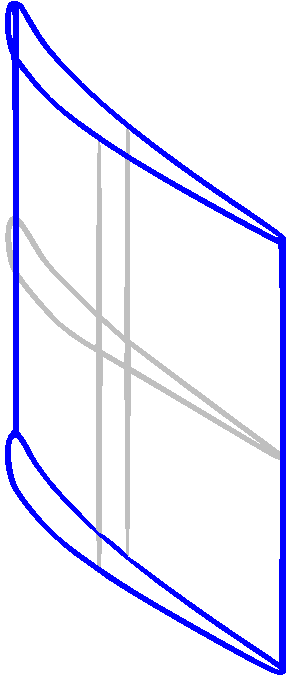
\includegraphics[height=.25\textheight]{img/original-blade.pdf}
  \caption{Original stator blade shape}
\end{subfigure}
\begin{subfigure}{.5\textwidth}
  \centering
  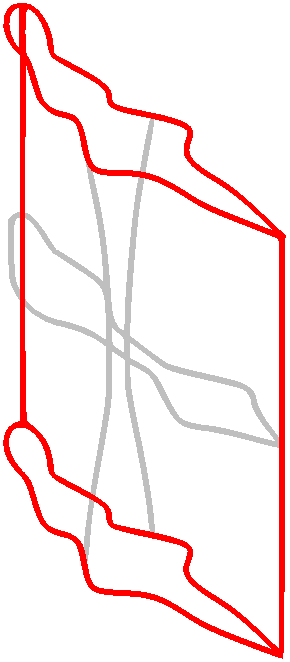
\includegraphics[height=.25\textheight]{img/target-blade.pdf}
  \caption{Perturbed stator blade shape}
\end{subfigure}
\caption{CAD optimisation with two stator blades}
\label{fig:drawtwoblades}
\end{figure}

% ##############################################
% The sections above show how to include figures and subfigures, how to label
% them, and how to cite them without remembering the figure number. Here 
% are two examples: (1) labeling: "\label{fig:drawtwoblades}" and citing:
% "\ref{fig:drawtwoblades}." LaTeX will do the rest for you.
% ##############################################

The primary objective of this test case is to match the surfaces of two blades by modifying the design parameters of the original blade. Since we have two versions of differentiated OCCT kernel, one compiled with \textit{traceless} and another one with \textit{trace-based} ADOL-C headers, the optimisation was performed twice.
We observed small differences between the gradients obtained from the two modes of AD, as shown in Fig.~\ref{fig:forwardvsreversecadonlygraddiff}.
Similar differences (same order of magnitude) were present in the primal results. We attribute the difference to floating-point round-off errors, since the floating point operations (and order) differ between \textit{traceless} and \textit{trace-based} ADOL-C headers. The differences relative to the objective function value, which is O($\cdot10^5$) are quite insignificant. The high peaks in differences occur, for example near gradient index $100$ (Fig.~\ref{fig:forwardvsreversecadonlygraddiff}), in the regions of low sensitivity values where round-off errors dominate.

The run-time ratios of the optimisation test-case for both forward and reverse mode AD are shown in Table~\ref{tab:computationaltimedifference}. Note that the run-time ratio is defined as the ratio between the original and differentiated OCCT sources. The \textit{trace-based} reverse mode AD is quite efficient and it is overall 47\% faster than the \textit{traceless} forward mode for the optimisation test-case.

\begin{figure}[h!]
 \begin{center}
  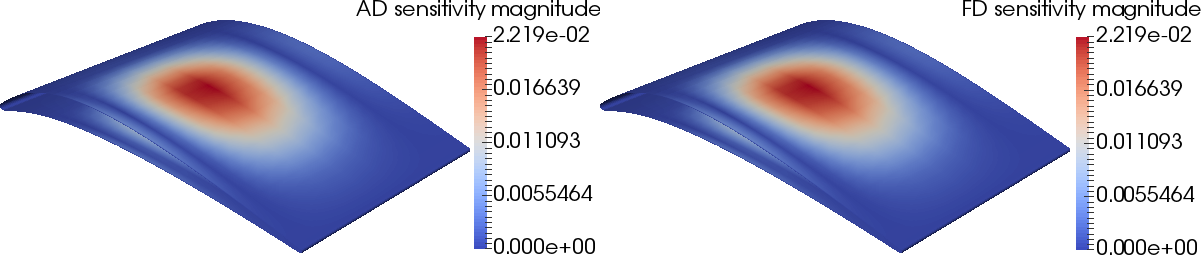
\includegraphics[scale=0.35]{img/ADvsFDparam150.png}
  \caption{Blade sensitivities evaluated by AD (left) and Finite Differences (right)}
  \label{fig:adfdsensitivity}
 \end{center}
\end{figure}

\begin{figure}
 \begin{center}
  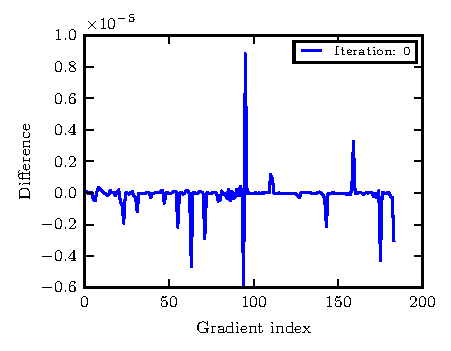
\includegraphics{img/ForwardVsReverseCADOnly_GradDifference.pdf}
  \caption{Gradient differences between two modes of AD for initial blade optimisation iteration}
  \label{fig:forwardvsreversecadonlygraddiff}
 \end{center}
\end{figure}

% #############################
% Below is an example of how to include a table.
% #############################

\begin{table}[h!]
\centering
\begin{tabular}{r|ccc}
& Original sources & AD Forward mode (traceless) & AD Reverse mode (trace-based)\\ \hline
Avg. time (seconds)& 0.09 & 13.27 & 6.99\\
Run-time ratio & & 147.44 & 77.67 
\end{tabular}
\caption{Timings for initial blade optimisation iteration done with original and differentiated (AD) sources}
\label{tab:computationaltimedifference}
\end{table}



\section{DIFFERENTIATED OCCT AND ADJOINT CFD COUPLING}
In a typical aerodynamic shape optimisation process one minimises a cost function $J$ (usually scalar like lift, drag, etc.) with respect to the CAD geometry with design parameters $\alpha$ and subject to geometry and flow constraints $R$ \cite{jameson88aerodynamic}:
\begin{equation}
\label{eq:cost-func}
\underset{\alpha}{min} \hspace{0.5em} J(U(X(\alpha)), X(\alpha), \alpha)
\end{equation}
\begin{equation}
\label{eq:NS}
R(U(X(\alpha)), X(\alpha)) = 0\:. 
\end{equation}
Equation \eqref{eq:NS} describes the flow field within the domain of interest by system of Reynolds-Averaged Navier-Stokes equations, with the state variable $U$ and a computational mesh coordinates $X$, which depend on design parameters $\alpha$. In case of large amount of design parameters (usually the case in industrial applications) the adjoint method proves to be computationally efficient and could be derived by application of a chain rule to the system \eqref{eq:cost-func}-\eqref{eq:NS} yielding:
\begin{equation}
\label{eq:sens}
\dfrac{dJ}{d\alpha}=\Big[ \frac{dJ}{dX} +\nu^Tf \Big]\frac{\partial X}{\partial \alpha}\:,
\end{equation}
where 
\begin{equation}
f = -\frac{\partial R}{\partial X}\:.
\end{equation}
Here $\nu$ represents the solution of adjoint equations:
\begin{equation}
\label{eq:adjoint}
\Big ( \frac{\partial R}{\partial U}\Big)^T\nu=\frac{\partial J}{\partial U}\:.
\end{equation}
After computing the solution of primal and adjoint equations \eqref{eq:NS},\eqref{eq:adjoint}, one can rewrite cost function gradient in terms of surface grid points derivatives:
\begin{equation}
\label{eq:surfSens}
\frac{dJ}{d\alpha}=\frac{dJ}{dX_S}\frac{dX_S}{d\alpha}\:.
\end{equation}
Here, the relation (spring analogy, inverse distance weighting) between volume and surface grid points displacement is used $X = X(X_S)$. 
The first term in \eqref{eq:surfSens}, usually called \textit{CFD sensitivity}, corresponds to the flow sensitivity in the surface grid points $X_S$. These derivatives could be calculated by several available CFD solvers that have implemented the adjoint method. In this work we use our in-house discrete adjoint solver STAMPS (previously \textit{mgopt}) \cite{xu2015thesis}. 

% ##################################
% The section above illustrates the true richness of LaTeX:
% mathematical typesetting. It is nearly impossible to beat
% LaTeX in this game.
% ##################################

The second term (\textit{CAD sensitivity}) represents the derivative of the surface grid points $X_S$ with respect to the CAD model design parameters. This part is calculated in the automatically differentiated version of OCCT \cite{auriemma2016optimisation}. The differentiated OCCT provides the derivatives for almost every possible CAD parametrisation and geometrical manipulation. 



Equipped with these derivatives, we compose them in the total gradient, which is then used in iterative gradient-based optimisation loop:
\begin{equation}
\label{eq:generalStep}
\alpha^{(n+1)} =  A\big(\alpha^{(n)}, \frac{dJ}{d\alpha}(\alpha^{(n)})\big) \:,\end{equation}
with $A$ as an optimisation algorithm. 
Next sections describe two cases of the above mentioned method, depending on the nature of CAD design parameter $\alpha$: as design variable in parametric CAD model or BRep/NURBS parametrisation.

\section{PARAMETRIC CAD-MODEL FOR TU BERLIN STATOR AND CONSTRAINTS}
\label{sec:paramtub}
The TUB TurboLab Stator Blade \cite{tubwebsite} is a typical turbomachinery optimisation testcase, where geometrical constraints strongly influence the final optimised shape. The test case prescribes the following geometrical constraints on the blade: (i) minimum radius of the leading and the trailing edge, (ii) minimum thickness of the blade (iii) minimum thickness near the hub and the shroud to accommodate the four mounting bolts and (iv) constant axial chord length. In the present work, we re-parametrised the blade in OCCT such that all constraints except the thickness constrains for the mounting bolts are explicitly embedded in the parametrisation. These constrains can readily be provided to any optimiser workflow.


\subsection{2D Profile Parametrisation}
The blade parametrisation starts by defining a 2d profile. We used B-spline curves to represent the 2d blade profiles, since they provide a rich and flexible space for the parametrisation \cite{verstreate2010cado}. The 2d blade profile is generated using a camber-line (shown in Fig.~\ref{fig:orestoption}) represented by a B-spline curve and characterised by seven control points. We distribute eight reference points $(P1,...,P8)$, as shown in Fig.~\ref{fig:orestoption}, along the camber line using a cosine function. The cosine function is used to cluster points near the leading and trailing edge (\textit{LE} and \textit{TE}) of the camber-line. The control points for the suction and pressure side B-splines curves are generated as equidistant offsets of the reference points normal to the camber-line (Fig. ~\ref{fig:orestoption}). Finally, the suction and pressure side curves are smoothly joined using the specified radius of curvature satisfying G2 continuity.


\begin{figure}[h!]
\centering
 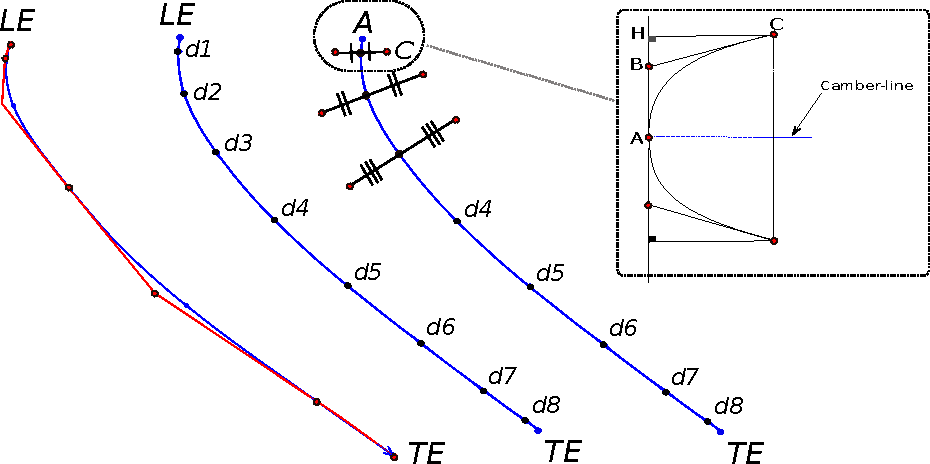
\includegraphics[height=.25\textheight]{img/salvi3.pdf}
\caption{Left: Camber-line (blue) with corresponding control polygon (red) and uniform point distribution; Right: Construction of pressure/suction control points; Imposition of curvature (G2 continuity) at the LE}
\label{fig:orestoption}
\end{figure}

\noindent
The AB length (Fig.~\ref{fig:orestoption}) in a B-spline curve of degree n is:

\begin{equation}
AB = \sqrt{curvature \cdot CH \cdot \frac{n-1}{n}}
\end{equation}

\noindent
where \textit{AB} is the distance between control point \textit{A} and \textit{B} and \textit{CH} is the distance of control point \textit{C} from the \textit{AB} line.
Therefore, it is possible to impose the curvature in the point \textit{A}.

This approach is applied to suction and pressure B-splines. In particular, the two curves have the same radius of curvature at the LE. This radius is controlled as design parameter of the optimisation. The same approach is also used for the TE radius. Thus the G2 continuity is kept along all the section. 

In summary, the 2d profile consists of 23 parameters of which, (i) 10 parameters control thickness (2 of them are the radii of TE and LE) and (ii) 13 parameters control the camber-line movement and, therefore, its angle, as shown in Fig.~\ref{fig:2dsection}.



\subsection{3D Parametrisation}
The 3d blade parametrisation is based on a cross-sectional design approach - the \textit{lofting}. This approach takes \textit{n}-slices (2d profiles) as input and constructs final B-spline surface using an OCCT approximation tool. The slices are generated along a blade span defined as a B-spline curve, the \textit{path-line}. Each 2d profile parameter is characterised by a law of evolution along the \textit{path-line}. The laws are defined as B-spline curves, consisting of 8 control points each. These control points are the design parameters of the optimisation. Their total number is 184 ($23 \cdot 8$). An example of the blade construction using seven slices is shown in Fig.~\ref{fig:Blade}.

% ##############################################
% Below is an example of how to put figures side by side using the "minpage"
% command. Smaller images should always be placed side by side.
% ##############################################

\begin{figure}
\centering
\begin{minipage}{.5\textwidth}
  \centering
  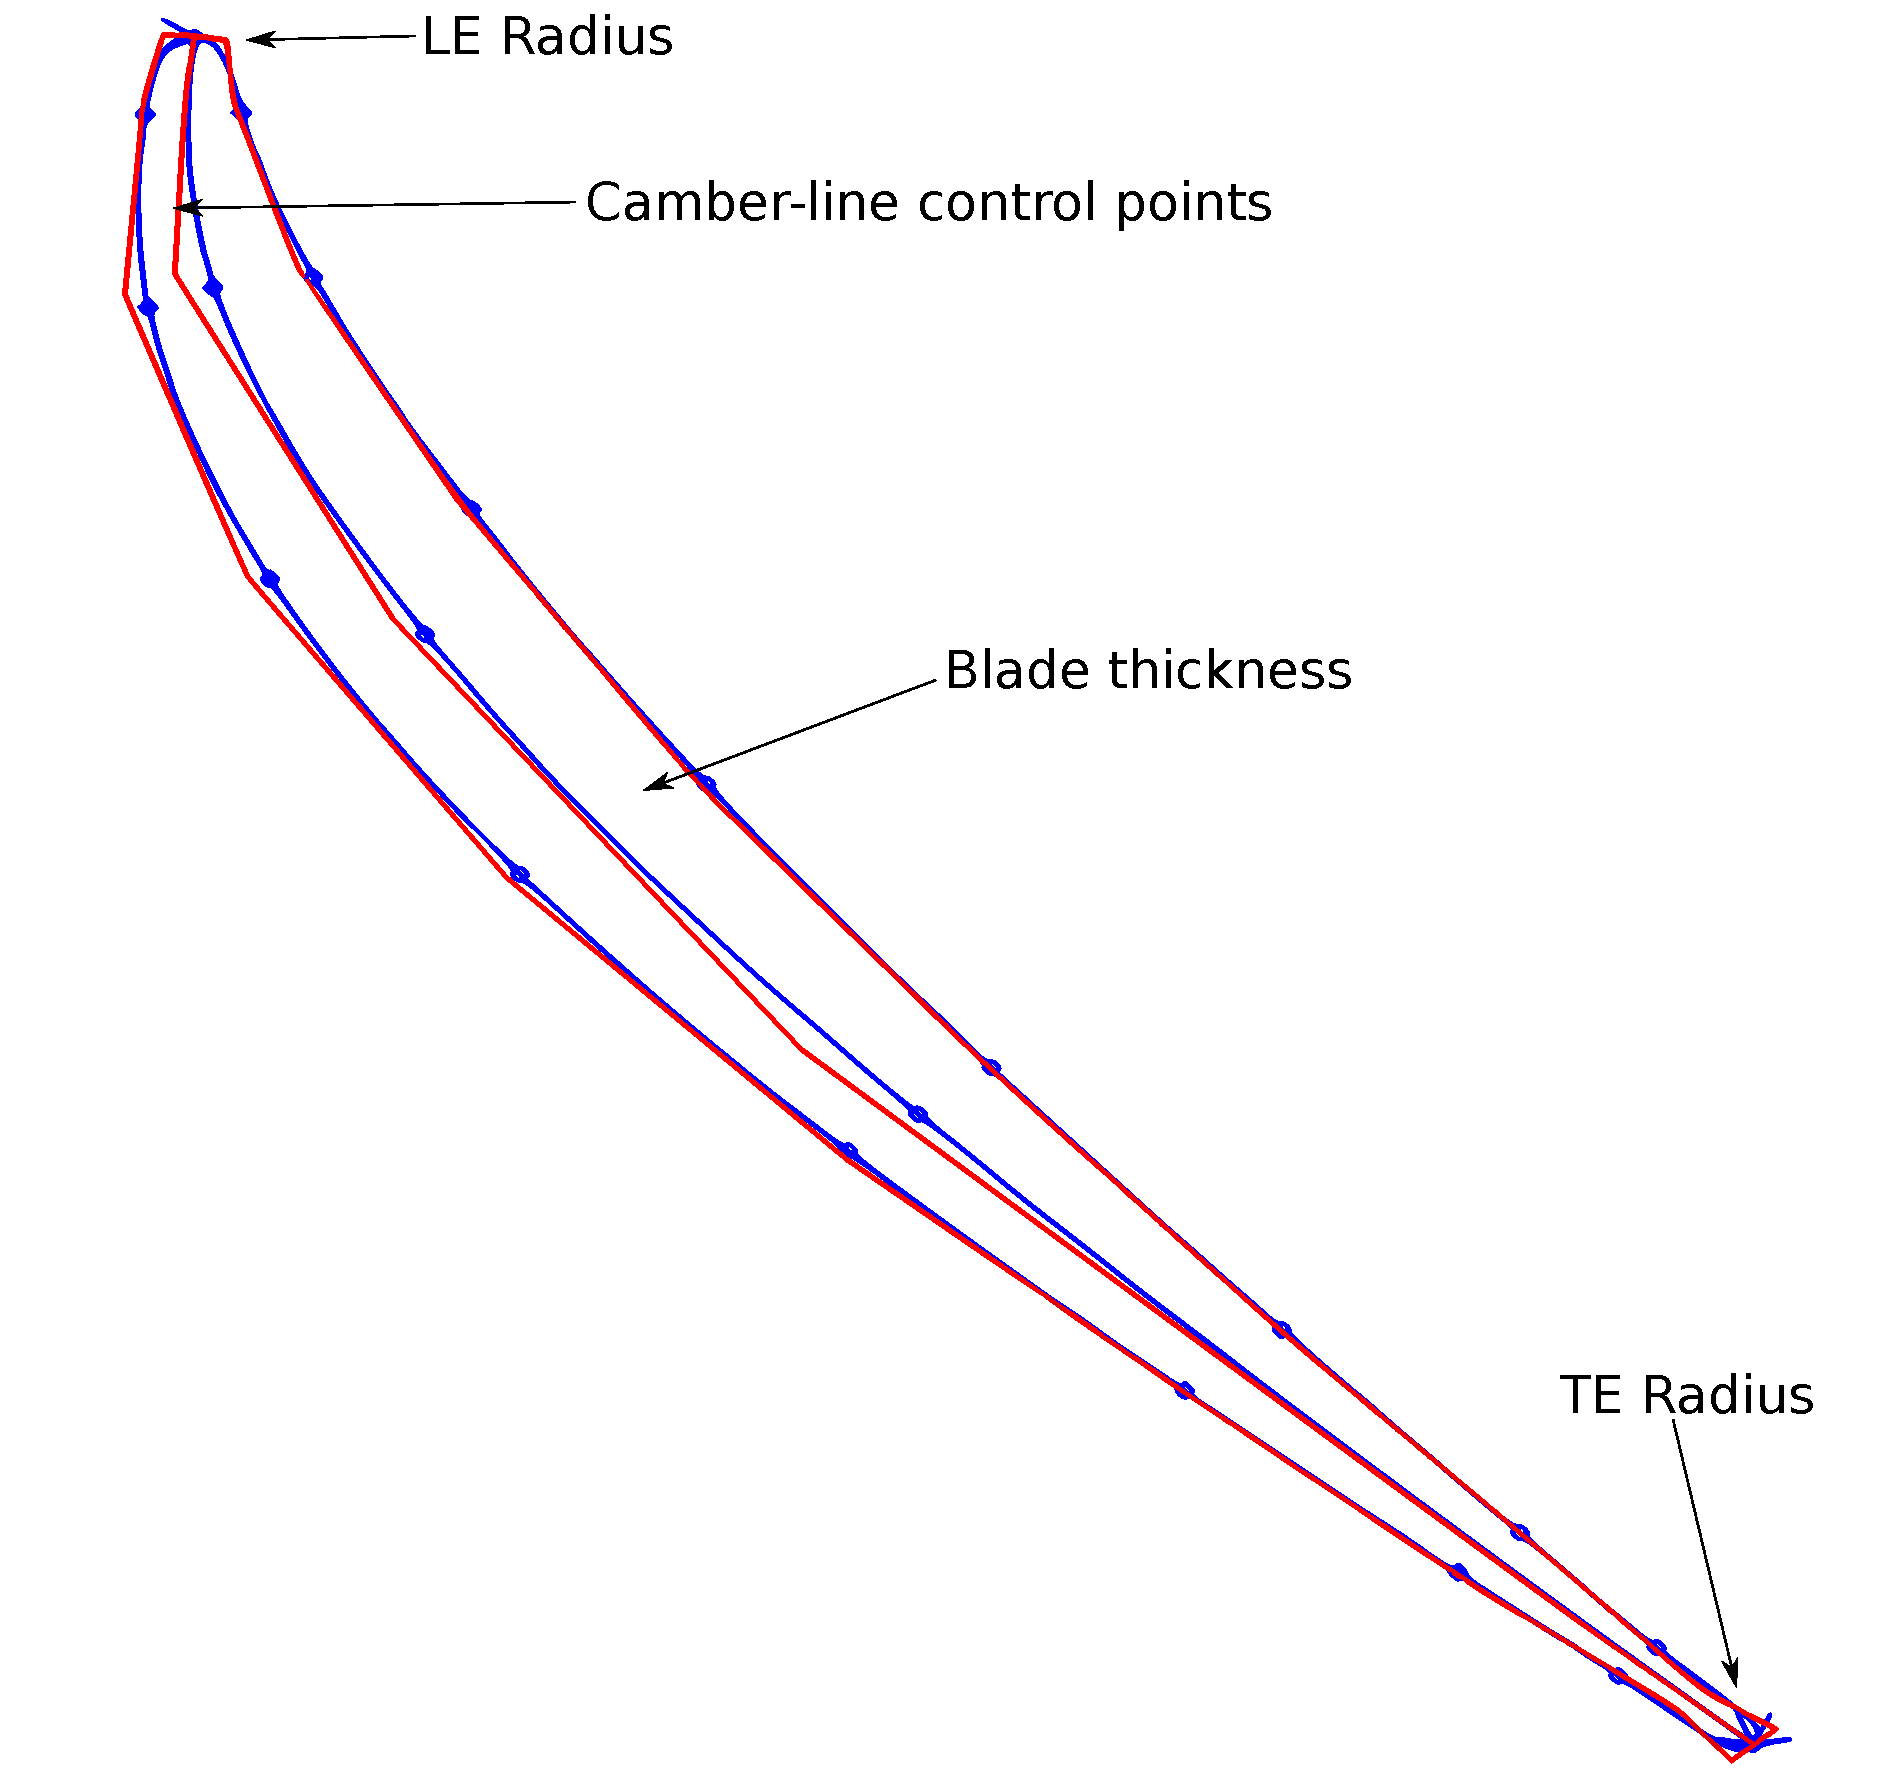
\includegraphics[scale=0.2]{img/sectionCosPic.pdf}
   \captionof{figure}{Section parameters}
   \label{fig:2dsection}
 \end{minipage}%
\begin{minipage}{.5\textwidth}
  \centering
 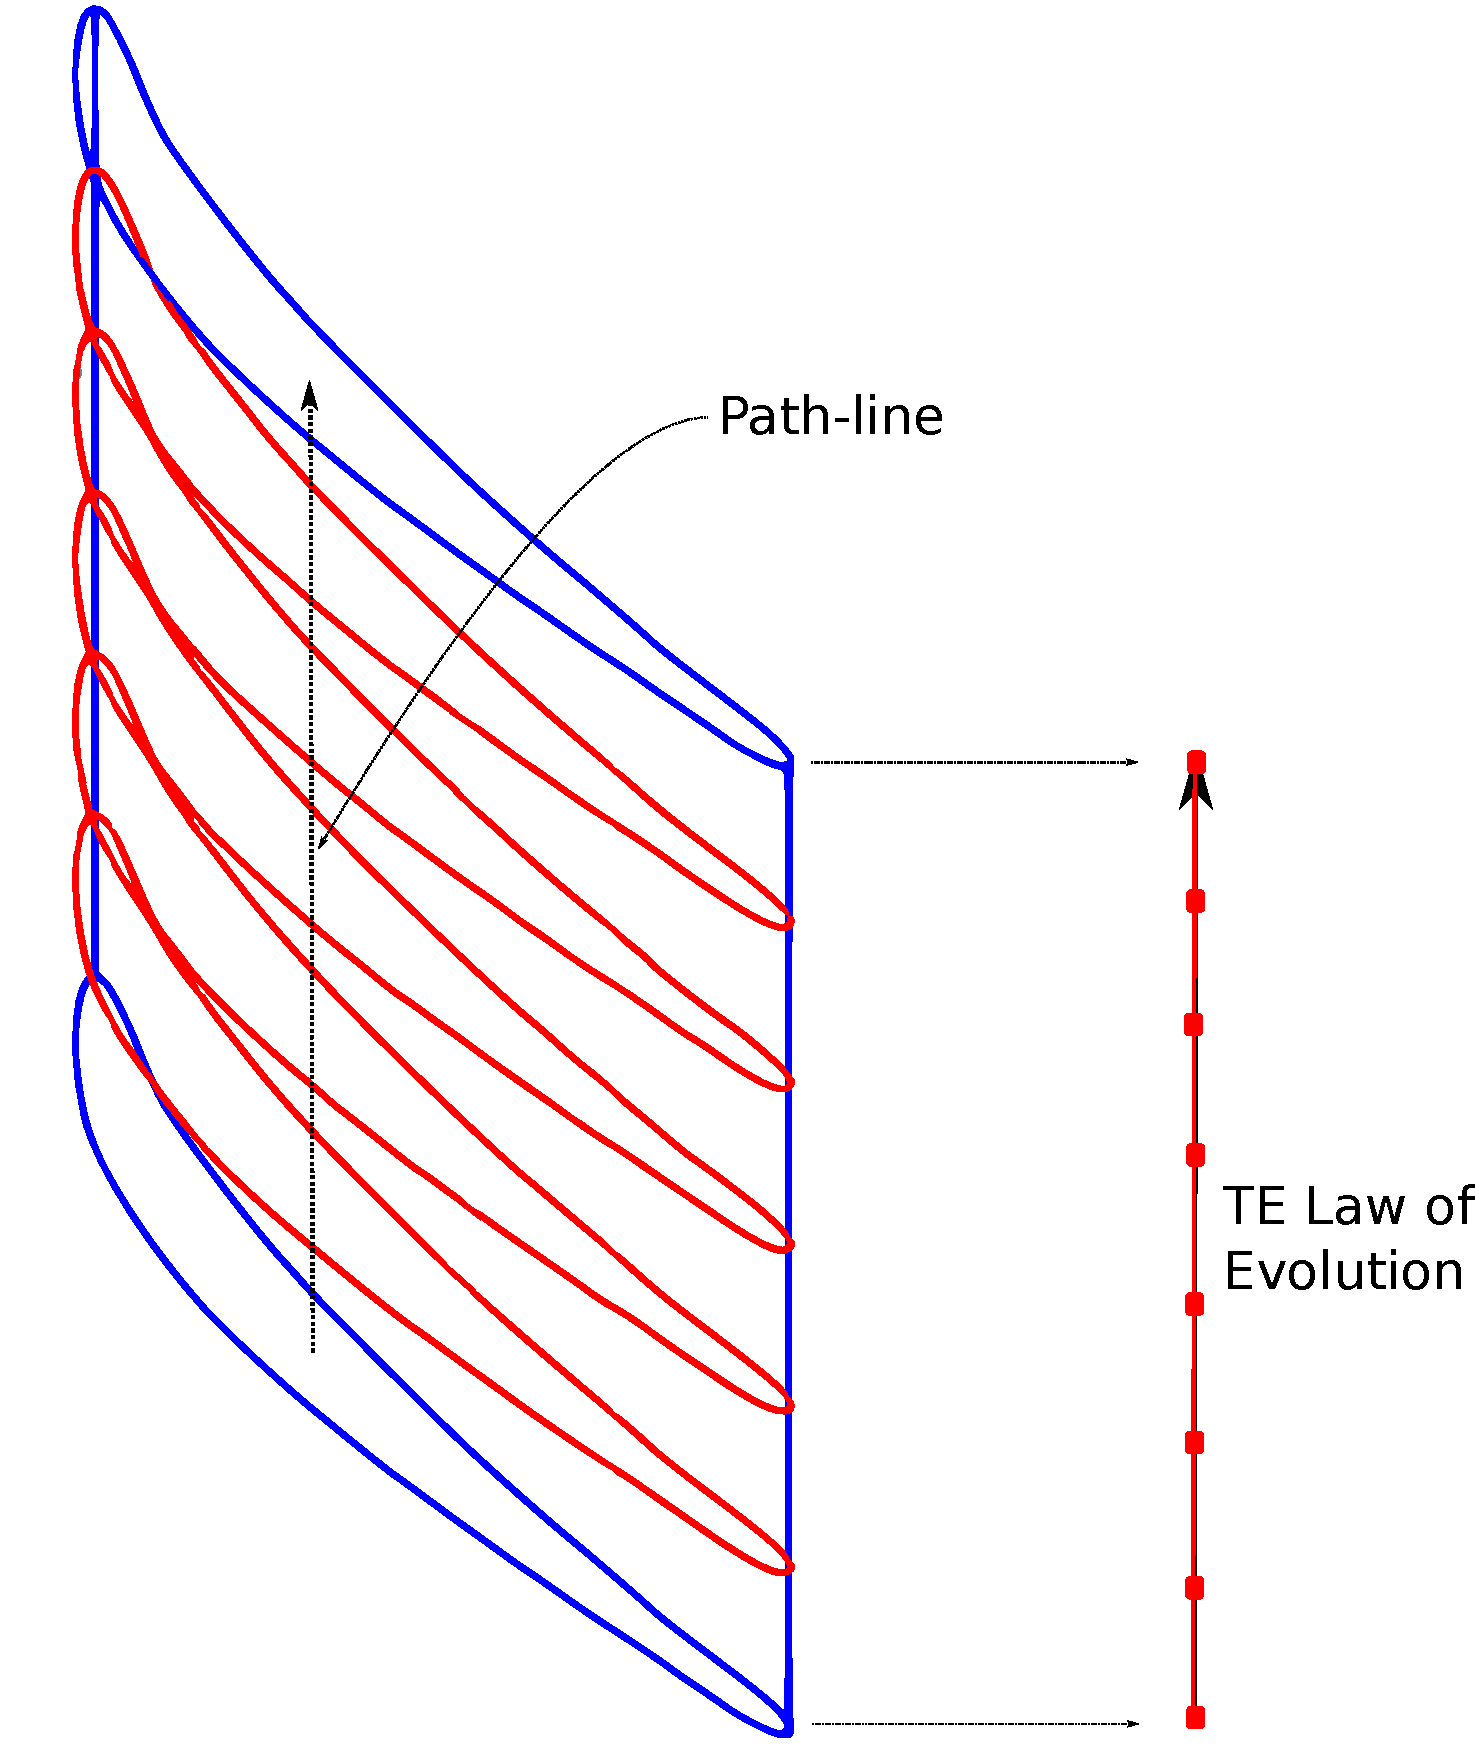
\includegraphics[scale=0.23]{img/blade2.pdf}
  \captionof{figure}{Blade skeleton and TE law of evolution in the 3D domain}
  \label{fig:Blade}
\end{minipage}
\end{figure}



\subsection{Optimisation Constraints}

The limited memory BFGS algorithm with boundary constraints (L-BFGS-B) is used as optimiser. The constraints specified in the L-BFGS-B are as follows:

\begin{itemize}[itemsep=0em]
\item G2 continuity: imposed along all the section based on the geometrical construction.
\item Axial chord: the axial-coordinate of the last camber-line control point is set equal to the axial-coordinate of the first control point plus the constant axial chord value.
\item Thickness distribution: the thickness between the suction and pressure surface is approximated using the corresponding B-Spline control point distances. Therefore this constraint has to be verified a posteriori.
\item LE and TE radii: The lower bound values are specified.
\end{itemize}

\section{NURBS-BASED OPTIMISATIONS AND CONSTRAINTS}
\label{sec:nurbs}
The NURBS-based optimisation technique with continuity and geometrical constraints (so-called NSPCC approach) was initially proposed in \cite{xu13:cad-based} and \cite{xu15cad-based}. In this paper, we extend and automate the NSPCC method further. The authors in \cite{xu13:cad-based} use a modest in-house CAD kernel, but we substitute it with a comprehensive OCCT CAD kernel and  benefit from the extensive CAD functionality. The major updates and novelties are related to the refinement of the CAD-space, new constraints capabilities (curvature), recovery of the violated geometrical constraints and the storage of the constraints in standard CAD formats. In the current NSPCC version the role of the CAD tool is more profound, while the amount of manual constraint set-up is reduced. This brings NURBS-based optimisation closer to the industrial workflows and creates an alternative to parametric CAD-models optimisation. 

\subsection{NURBS-based Design}
The advantage of NURBS-based approach is that in most cases no preprocessing (understanding of initial parametrisation tree, re-parametrisation in another tool, aerodynamic intuition to define proper CAD space, etc.) is needed. CAD-vendor neutral boundary representation could be retrieved directly from the standard CAD files (STEP, IGES, etc.), which usually contain collection of NURBS patches.

% ###########################
% Below is an example of how create a table.
% ###########################

Since OCCT is already equipped with an efficient reader of standard CAD formats, its differentiated version allows to compute the sensitivity information in any point of the surface with respect to control points position of governing NURBS. Therefore the CAD sensitivity defined in Eq.~\ref{eq:surfSens} is obtained for every surface:
\vspace{-1em} 
\newcommand{\mymatrix}[1]{\ensuremath{\left\downarrow\vphantom{#1}\right.\overset{\xrightarrow[\hphantom{#1}]{\text{\tiny{3 $\times$ N}}}}{#1}}}
\begin{equation}
\label{eq:nurbsSens}
\frac{\partial X_S}{\partial \alpha} =  
\frac{\partial X_S}{\partial P} =  
\text{\tiny{3 $\times$ M} }\mymatrix{\begin{pmatrix}
  \frac{\partial X_{S1}}{\partial P_1} & \frac{\partial X_{S1}}{\partial P_2} & \cdots & \frac{\partial X_{S1}}{\partial P_N} \\
       \vdots  & \vdots  & \ddots & \vdots  \\
         \frac{\partial X_{SM}}{\partial P_1} & \frac{\partial X_{SM}}{\partial P_2} & \cdots & \frac{\partial X_{SM}}{\partial P_N} 
        \end{pmatrix}} \:.
\end{equation}
Here $M$ and $N$ are the total number of surface mesh points $X_S$ and control points $P$ respectively. Moreover, with OCCT one can easily and intuitively refine design space by adding extra control points with knot insertion algorithm \cite{piegl2012nurbs}. This operation does not change the shape or degree of the surface, but establishes more local control due to local support properties of the splines. This is clearly visible in the changing pattern of the CAD sensitivities shown in Fig.~\ref{fig:knotted}. These very narrow sensitivities potentially could cope better with small flow features not 'visible' for more global parametric sensitivity (Fig.~\ref{fig:adfdsensitivity}).  
\begin{figure}[!h]
\begin{center}
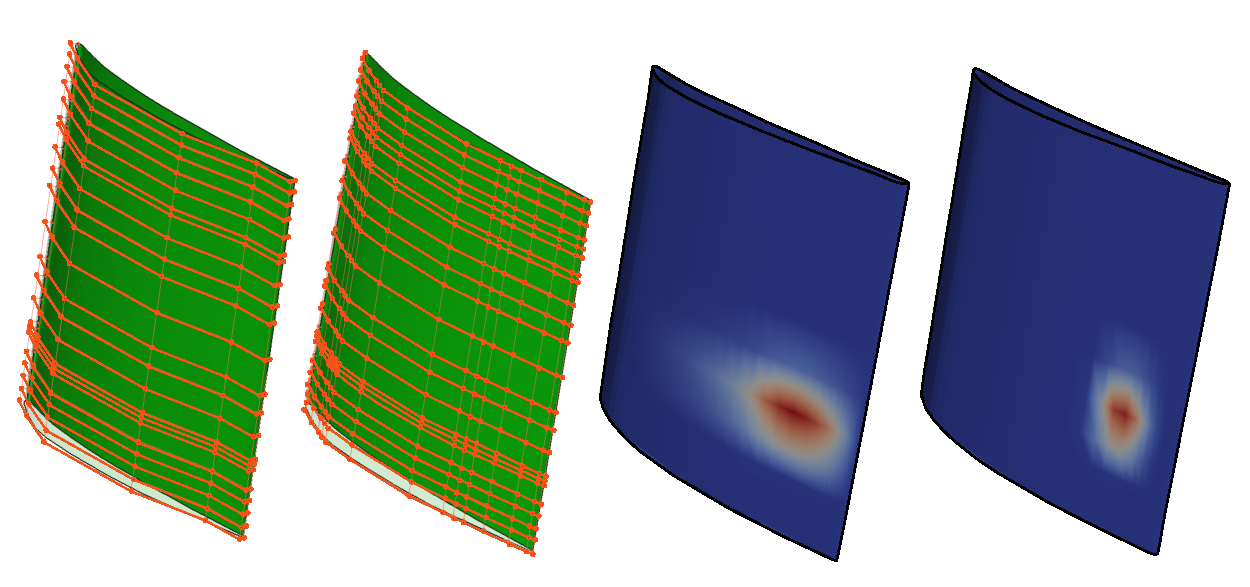
\includegraphics[width=0.8\textwidth]{img/knottedx12_paraviewSensPoled.pdf}
\caption{Left: Initial (9x22) and refined(18x22) Control Point Net of TUB Stator; Right: Corresponding changes in CAD Surface Sensitivity with respect to movement of the single control point}
\label{fig:knotted}
\end{center}
\end{figure}
At the moment, the refinement is performed manually prior to the optimisation, but this process can be automated with the CFD sensitivity field as a sensor for refinement.

It is important to note that in some cases the NURBS surfaces extracted from standard files are not suitable for direct NURBS-based optimisation due to enormous clustering of control points (sometimes as fine as the computational mesh). The root of this problem lies in the creation of the initial shape (morphed from STL, extensive surface trimming, etc.). In these cases reverse engineering and re-approximation of the surfaces might be required. 

\bigskip

\subsection{Constraints}

CAD models are usually constructed from multiple adjacent patches. Therefore, modifications of control points individually on patches can violate (i) patch-continuity (holes between the CAD faces, non-smooth shapes) or (ii) other geometrical constraints. We alleviate this problem by filtering out the shape modes with undesired constraints violations using discrete spaces constructed using test-points \cite{xu13:cad-based}. Conceptually, the approach requires that the constraints are satisfied on the particular set of points defined on the surface (test-points). We avoid distinguishing the continuity and the geometrical constraints by bringing them under one framework.


In the TUB stator test-case, several geometrical constraints are present and were introduced in the previous section. Several methods were devised to accelerate and automate the process of test-point distribution. Firstly, we identify topological entities (e.g. edges, parts of surfaces, etc.) necessary for constraint imposition. For instance, to distribute test-points along the leading edge (curvature and continuity constraints), we use OCCT to find two parametric curves (\textit{PCurves}) of the edge on two adjacent faces (Fig.~\ref{fig:pcurves}). Then we use OCCT to uniformly distributes points (in $1d$ parametric space) along each \textit{PCurve}. As a result two pairs of test-points are generated each belonging to the respective \textit{PCurves}. The test-point pairs along the \textit{edge1} (LE) and \textit{edge2} (TE) are then used to impose continuity and curvature constraints. It is also possible to generate test-point pairs on \textit{PCurves} at arbitrary location on a given patch face (connect the predefined endpoints $(u1,v1)$ and $(u2,v2)$ in the parametric space of the face). The generated test-points pairs are then used to impose thickness constraints between the two patches of the Stator. The treatment of constraints on a topological level allows to store these \textit{PCurves} in a standard CAD file. This enables visualisation and inspection of the constraints during optimisation. For example in Fig.~\ref{fig:constraints} the pairs of \textit{PCurves} are shown, where \textit{PCurves} pairs are identically coloured. In addition, the \textit{PCurves} can be stored and visualised as wire-frame objects with vertices as test-points.

\begin{figure}
\begin{center}
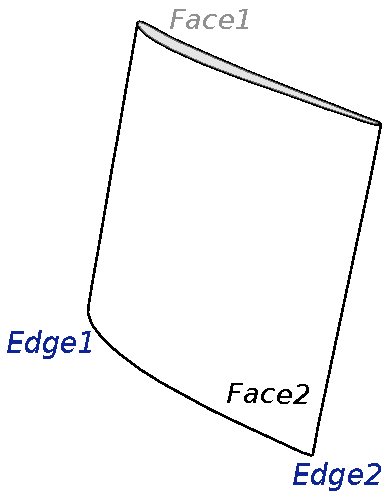
\includegraphics[width = 0.18\textwidth]{img/topo.pdf}
~~
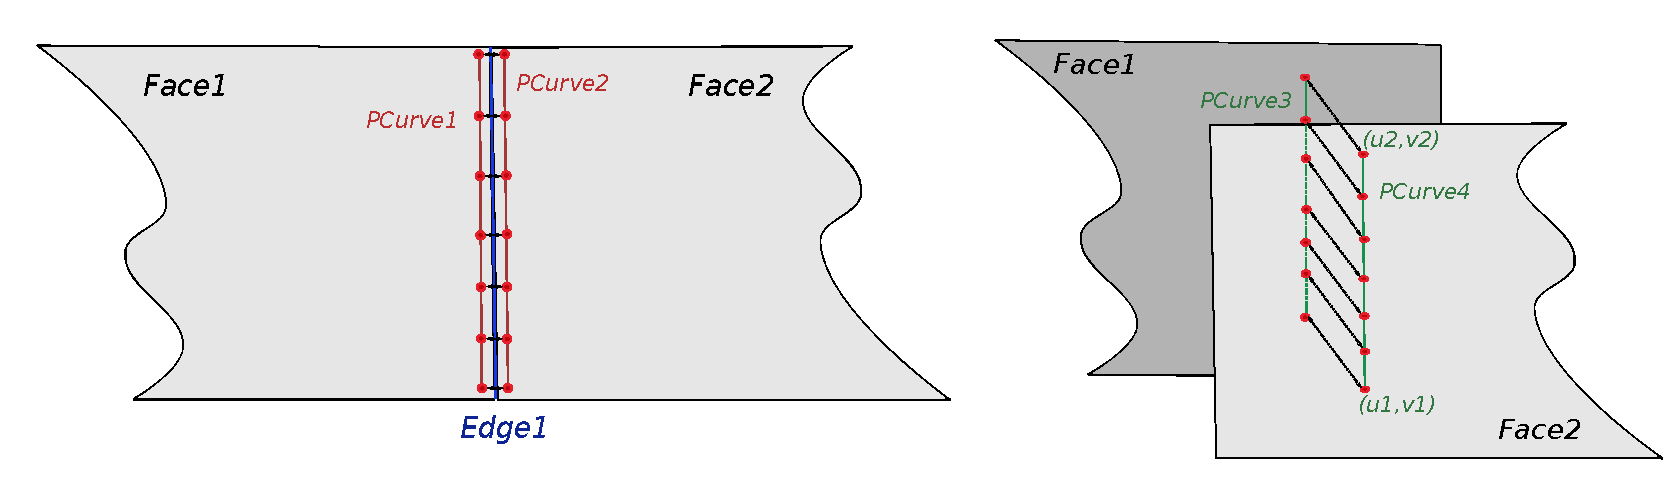
\includegraphics[width = 0.75\textwidth]{img/faceTP2.pdf}
\caption{Left: TUB Stator Topology; Middle: Test-points distribution along \textit{PCurves} of the common edge; Right: Test-points on generic \textit{PCurves} of surfaces}
\label{fig:pcurves}
\end{center}
\end{figure}
\begin{figure}
\begin{center}
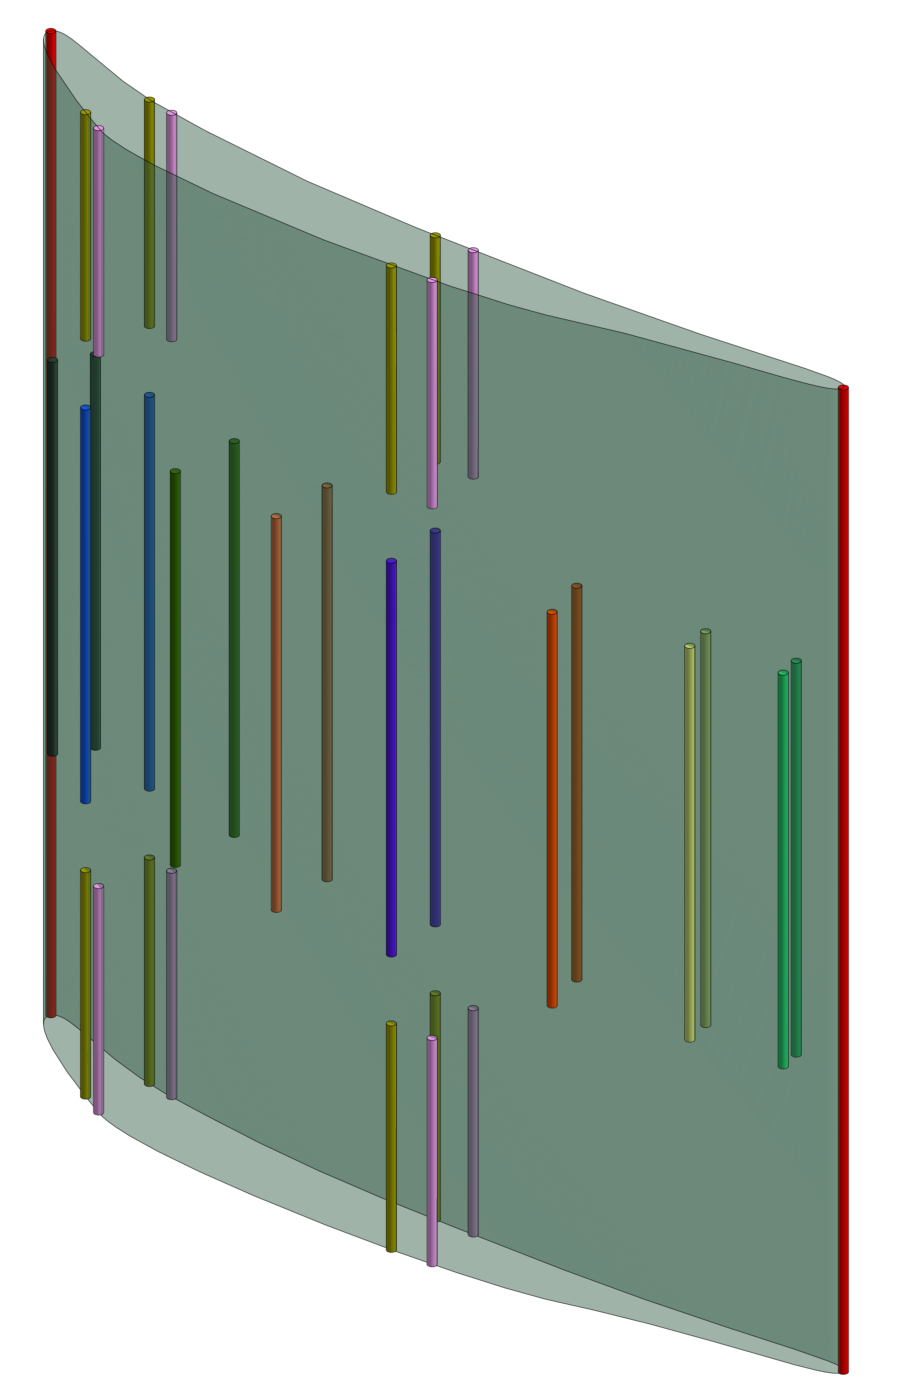
\includegraphics[width = 0.3\textwidth]{img/NewCylindersC1.pdf}
~~

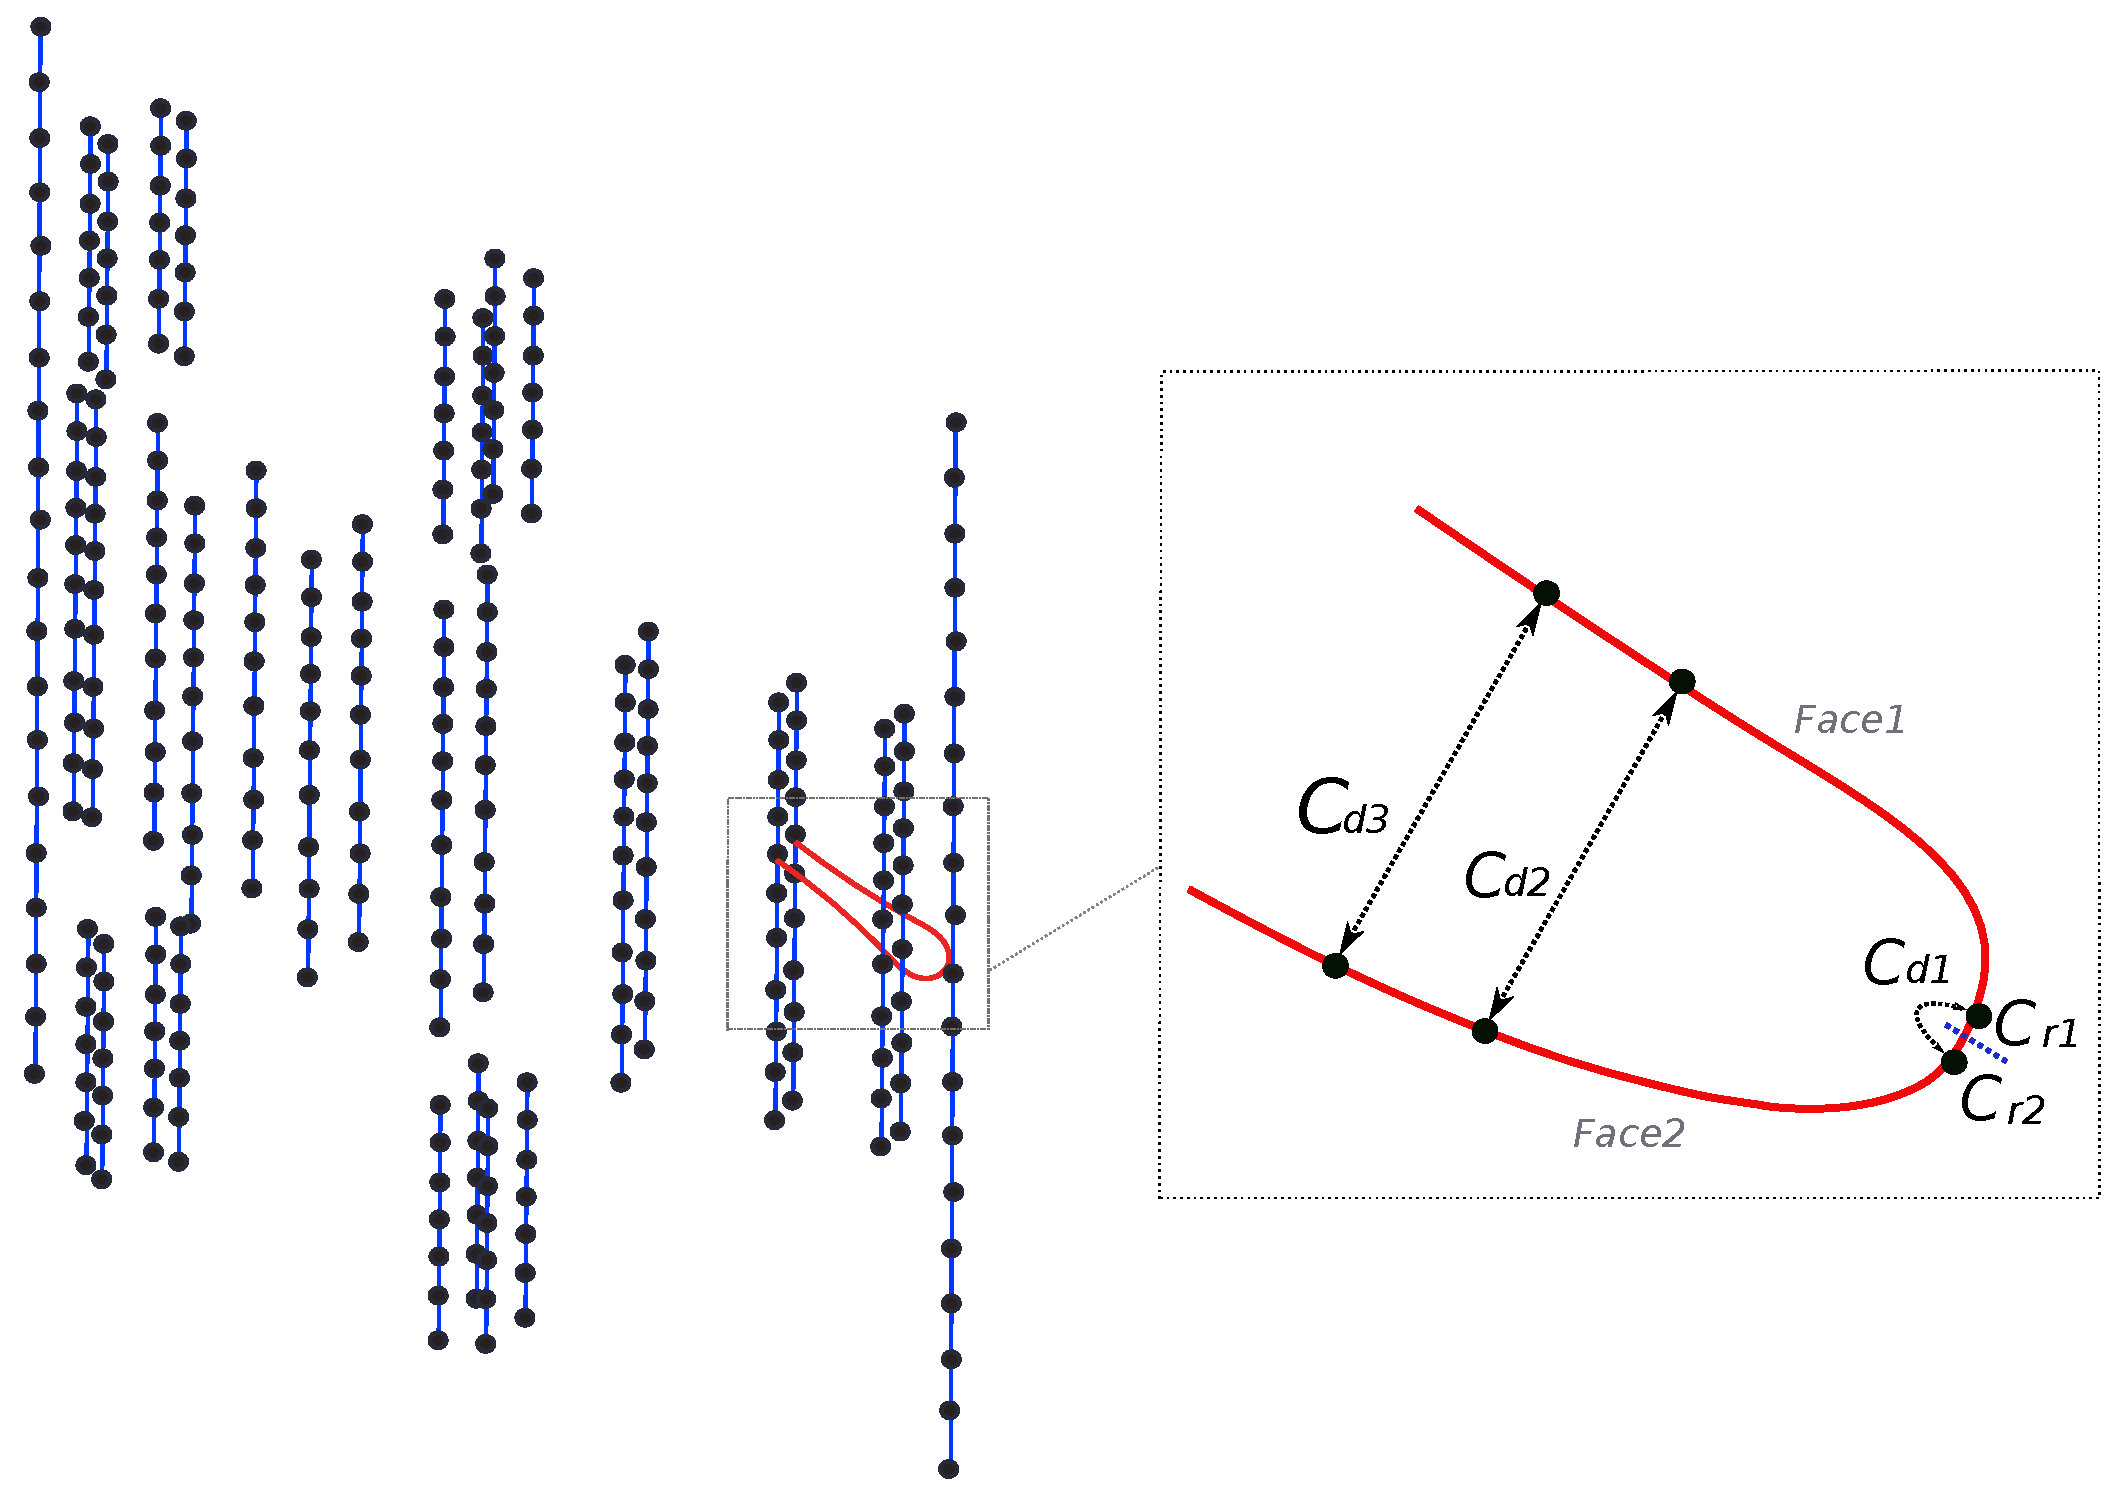
\includegraphics[width = 0.6\textwidth]{img/const3.pdf}
\caption{Left: Constraint visualisation from the STEP file; Right: Constraints computation on the testpoints}
\label{fig:constraints}
\end{center}
\end{figure}

Once all necessary test-points are distributed, standard OCCT geometric algorithms (\textit{distance, curvature, normal, etc.}) can be used to compute the following constraints:
\begin{itemize}[itemsep=0em]
\item Distance constraints\\
To fix the distance $d_r$ between two test-points ($X_{t1}, X_{t2}$), the following function is constructed:
\begin{equation}
C_{d} = distance(X_{t1}, X_{t2}) - d_r = 0\:.
\end{equation}
This constraint is used to ensure $G0$  continuity ($d_r = 0$ is then used) and the constant axial chord length. Similarly, the minimum thickness ($T_{min}$) constraint, which is required in the middle of the blade and for the bolts, corresponds to inequality constraint and is represented with:
\begin{equation}
\label{eq:din}
C_{d} = 1 - min\big(1,\frac{distance(X_{t1}, X_{t2})}{T_{min}}\big) = 0\:.
\end{equation}
\item Radius of curvature constraint\\
OCCT allows to compute minimum and maximum curvature in any point of the surface. Therefore, the radius in the test-point corresponding to TE and LE can be calculated as $r = 1/curvature(X_{t1})$. Constraint function bounding the minimum radius value to $(r_{min})$ is:
\begin{equation}
\label{eq:rad}
C_{r} = 1 - min\big(1,\frac{r}{r_{min}}\big) = 0\:.
\end{equation}

\item Smoothness constraint
\\G1 continuity can be imposed as:
\begin{equation}
C_s = normal(X_{t1}) \times normal(X_{t2}) =0 \:. 
\end{equation}
\end{itemize}
The $min$ operator in Eq.~\ref{eq:din} and Eq.~\ref{eq:rad} is used to 'activate' inequality constraint if it gets violated, and 'deactivate' it (constraint value is zero) otherwise. With differentiated OCCT we assemble derivatives of all constraint-functions into the constraint matrix:
\vspace{-1em} 
\newcommand{\myxmatrix}[1]{\ensuremath{\left\downarrow\vphantom{#1}\right.\overset{\xrightarrow[\hphantom{#1}]{\text{\tiny{T}}}}{#1}}}
\begin{equation}
\label{eq:nurbsSens}
C =  
\frac{\partial C_x}{\partial P} =  
\text{\tiny{3 $\times$ N} }\myxmatrix{\begin{pmatrix}
  \frac{\partial C_{d1}}{\partial P_1} & \frac{\partial C_{d2}}{\partial P_1} &  \cdots & \frac{\partial C_{cr1}}{\partial P_1} & \frac{\partial C_{cr2}}{\partial P_1} & \cdots & \frac{\partial C_{cr}}{\partial P_1} \\
        \vdots  & \vdots  & \ddots & \vdots  & \vdots  & \ddots & \vdots  \\
          \frac{\partial C_{d1}}{\partial P_N} & \frac{\partial C_{d2}}{\partial P_N} &  \cdots & \frac{\partial C_{cr1}}{\partial P_N} & \frac{\partial C_{cr2}}{\partial P_N} & \cdots & \frac{\partial C_{cr}}{\partial P_N} \\
        \end{pmatrix}} \:.
\end{equation}
Here T correspond to the number of all above-mentioned constraints. Afterwards, the constraint matrix is used in the finite step update:
\begin{equation}
\label{eq:fstep}
P^{n+1} = P ^{n} +t \cdot Ker(C)\Big [(\nabla J) Ker(C)\Big]^T \:,
\end{equation}
where 
\begin{equation}
\nabla J =  \frac{\partial J}{\partial X_S} \frac{\partial X_S}{\partial P} \:.
\end{equation}
The last equation is equivalent to one step of a projected gradient method with a step size of $t$. Here $Ker(C)$ is the kernel of the constraint matrix. This ensures that the control point perturbations are in the null space of the constraint matrix i.e., control points are modified without violating the constraints (at least for infinitesimal step-size).

\subsection{Constraint Recovery}
Due to non-linearity of constraints (G1, curvature) and inequality constraints (some constraints are inactive) they could be violated after the finite step - Eq.~\eqref{eq:fstep}. To overcome this, we have extended the continuity recovery method proposed previously in \cite{xu13:cad-based} to all type of constraints. 

First, by means of OCCT we indicate constraints that are indeed violated ($|\delta G_{d,r,s}| = |C_{d,r,s}| > \epsilon$) and input them into violation vector $\delta G_{violated} = (\delta G_1, ...,\delta G_{N_{violations}})$. We decompose constraint matrix into two matrices $C = C_{violated} \cup C_{satisfied}$ with columns entries corresponding to violated or satisfied constraints respectively. Afterwards, the necessary control point update could be defined: 
\begin{equation}
C_{violated} {\delta}P_{upd} + {\delta}G_{violated} = 0 \:,
\end{equation}
which also have to satisfy the rest of the constants:
\begin{equation}
{\delta}P_{upd} = Ker (C_{satisfied}) \delta {\alpha}\:,
\end{equation}
where $\alpha$ corresponds to the coefficients of linear combination of null space vectors.
This could be further developed as: 
\begin{equation}
{\delta}P_{upd} = -  Ker (C_{satisfied}) {\big[ C_{violated}  Ker (C_{satisfied})\big]}^{+} {\delta}G_{violated}\:.
\end{equation}
Here, superscript $^+$ corresponds to the pseudoinverse of rectangular matrix and usually only few Newton steps are needed to recover constraints.  
The implications of this approach goes beyond shape optimisation and could be applied directly on CAD shapes, which does not satisfy some certain requirements. We have used the TUB stator model with TE radius $r = 0.7$ and imposed minimum curvature/radius constraint there $r = 1$. This created constraints violations corresponding to every test-point located on the TE. Results of the recovery step with single Newton step are shown in Fig.~\ref{fig:recovery}, with all constraints satisfied for the updated red surface. 
\begin{figure}[!ht]
\begin{center}
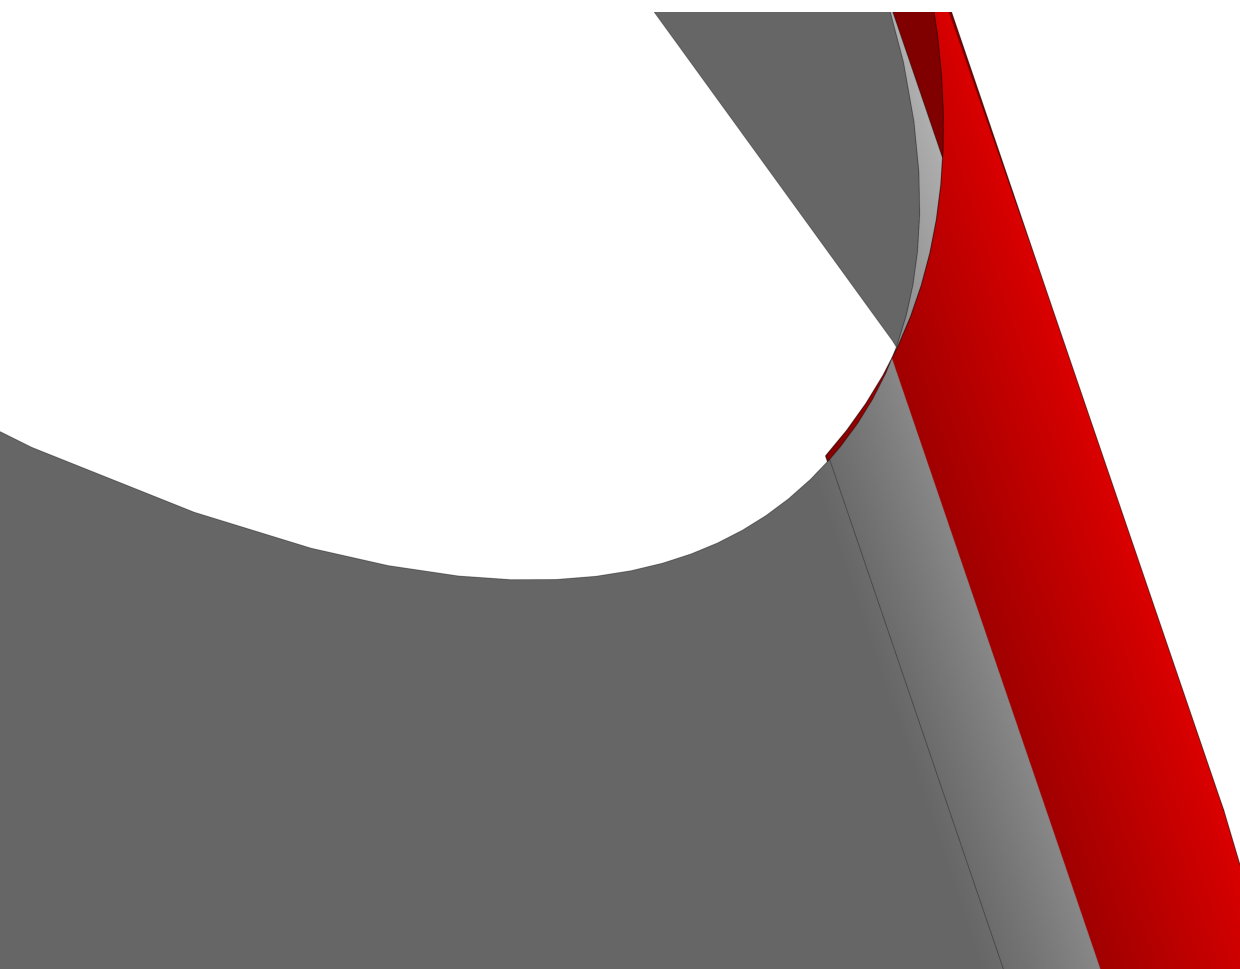
\includegraphics[width = 0.4\textwidth]{img/UpdatedCurvature.pdf}
\caption{Recovery/Increase of TE radius from initial (grey) to updated (red)}
\label{fig:recovery}
\end{center}
\end{figure}

\section{AERODYNAMIC SHAPE OPTIMISATION OF TU BERLIN STATOR}
\label{sec:results}

\subsection{Optimisation Workflow}
This subsection summarises the main steps that we use for redesign of the TU Berlin Stator. The algorithm is generic and can be applied without major changes to any other aerodynamic shape optimisation problem. To set up a new test-case, one has to provide new parametrisation and the corresponding CFD mesh. We refer to two aforementioned parametrisation as a) for parametric and b) for BRep. Both of them could be used in two distinct optimisation procedures: 
\begin{enumerate}
\item Define parametrisation and design surfaces.
\item Perform mesh point inversion (find mesh points $X_S$ that belong to the design surfaces).
\item Run primal and adjoint CFD (get cost function value), compute CFD sensitivity: $\frac{dJ}{dX_S}$.
\item Compute CAD sensitivity $\frac{dX_S}{d\alpha}$ depending on the chosen parametrisation:
\begin{enumerate}[label*=\alph*)]
\item parametric approach: use differentiated OCCT to get sensitivities w.r.t the explicit design parameters (Sec.~\ref{sec:paramtub});
\item NURBS-based approach: use differentiated OCCT to compute gradients w.r.t. the control points positions and to construct corresponding constraint matrix $C$ (Sec.~\ref{sec:nurbs}).
\end{enumerate}
\item Compose total gradient $\frac{dJ}{d\alpha} = \frac{dJ}{dX_S} \frac{dX_S}{d\alpha}$.
\item Update design parameters using  $\frac{dJ}{d\alpha}$, change CAD geometry and corresponding mesh:
\begin{enumerate}[label*=\alph*)]
\item update design parameters using L-BFGS-B optimiser. Geometrical constraints are automatically satisfied and lie within prescribed bounding values (Eq.~\ref{eq:generalStep});
\item update control points positions. Geometrical constraints are satisfied due to the projected gradient. Constraint matrix 'filter' ensures updates do not violate constraints (Eq.~\ref{eq:fstep}). 
\end{enumerate}
\item Repeat 3-6 until no further cost function improvement is possible.
\item Retrieve the optimised shape directly in the CAD format.
\end{enumerate}

\subsection{Optimisation Results}
The main focus of this paper is to demonstrate a feasible approach to include a complex  CAD model in a gradient-based optimisation chain. At this stage we use low-fidelity CFD simulations, but without any limitation this allows to test and demonstrate the strength of both aforementioned CAD parametrisations in the design chain, however restrain us from the detailed discussions on the physics of the initial and optimised flow results. Therefore, we generated a coarse computational grid with ICEM CFD from the existing CAD model and used it for flow simulations in the STAMPS solver. 

We perform two optimisations (explicit Parametric-based and implicit NURBS-based) to minimise the total pressure losses between the inlet and the outlet of the TU Berlin Stator. Two different optimisers were used, L-BFGS-B for the explicit and Steepest-Descent (with projected gradient) for the implicit parametrisation. The corresponding optimised CAD models are shown in Fig.~\ref{fig:optimised} together with the initial shape. In both cases we observe similar patterns of decrease of the 
leading edge and trailing edge radius and reduction of the blade thickness, while all geometrical constraints are satisfied. The optimised parametric and NURBS models improve the cost function by 14\% and 13\% respectively.
\begin{figure}[!h]
\begin{center}
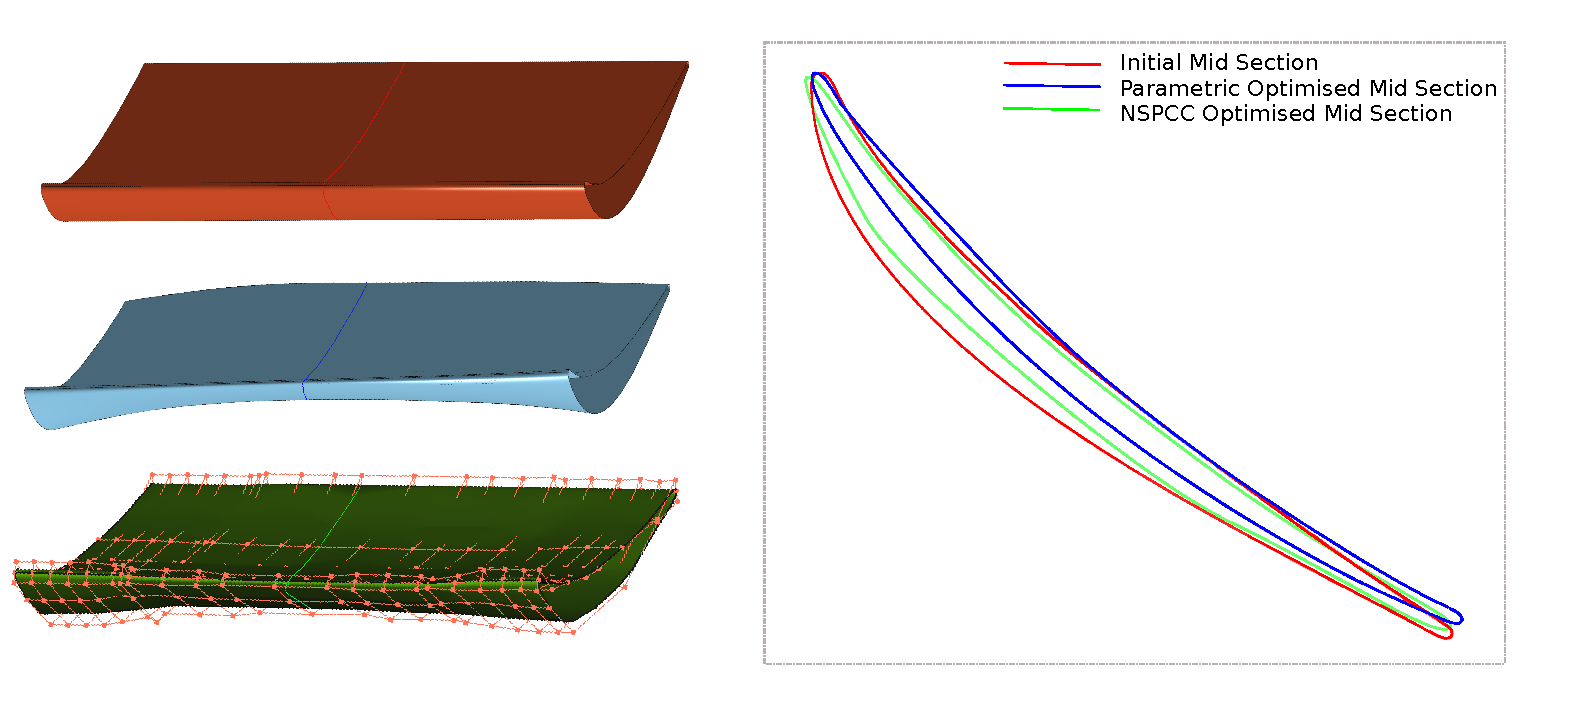
\includegraphics[width = 0.95\textwidth]{img/horisontal.pdf}
\caption{Left: Initial TU Stator (red), Optimised Parametric model (blue) and Optimised NURBS (green); Right: Comparison of mid-sections}
\label{fig:optimised}
\end{center}
\end{figure}


As highlighted in the comparison (Fig.~\ref{fig:optimised}) at the mid-section, the two optimised shapes are different, which originates from the differences in parametrisations and constraints. Judging by the CAD sensitivities (NURBS space generates very local sensitivities) the NUBRS-based approach could actually provide superior results. But contrary to the parametric model, it includes additional constraints for the mounting bolts. This results in a thicker blade towards the shroud and hub ends of the blade where the bolts are located. The imposition of identical constraints and use of high-fidelity CFD (increases the impact of CAD sensitivity locality) could enable further investigation of the occurring differences between two parametrisations.



\section{CONCLUSIONS}

We have successfully demonstrated the integration of a large-scale CAD system into the design chain 
for shape optimisation of immersed bodies. The OCCT CAD kernel that is algorithmically differentiated to compute shape derivatives is the cornerstone ingredient: it provides the  necessary CAD sensitivities efficiently, accurately and robustly. The approach allows to maintain CAD-models throughout the optimisation loop thus enabling work in a multi-disciplinary framework. In addition to aerodynamic shape optimisation, the coupling of the differentiated OCCT with structural analysis, conjugate heat transfer and robust design problems will be investigated in the future. The derivative information available in OCCT is also useful in a purely CAD context: (i) re-parametrisation of the models (formulated as the optimisation problem that tweaks parameters values to find the best 'fit' to the target geometry); (ii) recovery of the violated geometrical constraints.


Two different parametrisation techniques for aerodynamic shape optimisation of an industrial turbomachinery blade were proposed. For both of them the recipes for imposing manufacturing (geometrical) constraints were detailed. The storage of constraints in the standard CAD files and hence their visualisation and inspection is possible for the NURBS-based approach. The choice of either of the parametrisation for optimisation of an arbitrary CAD-model is case-dependent, since both approaches perform design explorations in the different spaces. The parametric CAD models are useful for the applications when decent parametrisations are well established through the previous engineering experience. The NURBS-based approach could then serve as the complementary or the alternative technique which is advantageous for the optimisation of non-conventional components.

\section*{ACKNOWLEDGEMENTS}
This research is a part of the IODA project - Industrial Optimal Design using Adjoint CFD. IODA is \textit{Marie Sklodowska-Curie Innovative Training Network} funded by European Commission under Grant Agreement No.~642959.

\bigskip
%\section*{ORCID}
\orcid{First M. Last,}{000-0002-1234-5678}
\orcid{First M. Last,}{000-0002-1234-5678}
\orcid{First M. Last,}{000-0002-1234-5678}   

% #########################################
% Please pay close attention to the formatting of the references:
%    Authors: Smith, J.; Doe, M.; White, K.:
%    Paper: listed as published
%    Journal: listed in its conventional name
%    Volume: 27(3), 2009, 123-130, i.e. volume, issue, year and pages
%    Conference: name, location, year, pages
%    DOI: https://doi.org/DOI number. You can get the entire link from
%    "https://doi.crossref.org/simpleTextQuery/"
%    Books: author(s), title, publisher, location, year
%    Website: title (if any) and full URL link
% ##########################################

\referenceSection
\bibliographystyle{CADA}
\bibliography{CADandA_Paper_Template}




\bigskip
\end{document}
